%%%%%%%%%%%%%%%%%%%%%%%%%%%%%%%%%%%%%%%%%
% Short Sectioned Assignment
% LaTeX Template
% Version 1.0 (5/5/12)
%
% This template has been downloaded from:
% http://www.LaTeXTemplates.com
%
% Original author:
% Frits Wenneker (http://www.howtotex.com)
%
% License:
% CC BY-NC-SA 3.0 (http://creativecommons.org/licenses/by-nc-sa/3.0/)
%
%%%%%%%%%%%%%%%%%%%%%%%%%%%%%%%%%%%%%%%%%

%----------------------------------------------------------------------------------------
%	PACKAGES AND OTHER DOCUMENT CONFIGURATIONS
%----------------------------------------------------------------------------------------

\documentclass[paper=a4, fontsize=11pt]{scrartcl} % A4 paper and 11pt font size

\usepackage{listings}
\usepackage{color}

\definecolor{dkgreen}{rgb}{0,0.6,0}
\definecolor{gray}{rgb}{0.5,0.5,0.5}
\definecolor{mauve}{rgb}{0.58,0,0.82}

\lstset{frame=tb,
language=Java,
aboveskip=3mm,
belowskip=3mm,
showstringspaces=false,
columns=flexible,
basicstyle={\small\ttfamily},
numbers=none,
numberstyle=\tiny\color{gray},
keywordstyle=\color{blue},
commentstyle=\color{dkgreen},
stringstyle=\color{mauve},
breaklines=true,
breakatwhitespace=true,
tabsize=3
}

\usepackage[T1]{fontenc} % Use 8-bit encoding that has 256 glyphs
\usepackage[utf8]{inputenc}
\usepackage[spanish]{babel} % English language/hyphenation
\usepackage{amsmath,amsfonts,amsthm} % Math packages
% \usepackage{breakcites}
\usepackage{sectsty} % Allows customizing section commands
\allsectionsfont{\centering \normalfont\scshape} % Make all sections centered, the default font and small caps
\usepackage{algorithm}
\usepackage{url}
\usepackage[noend]{algpseudocode}
\makeatletter
\usepackage{graphicx}

\usepackage{fancyhdr} % Custom headers and footers
\pagestyle{fancyplain} % Makes all pages in the document conform to the custom headers and footers
\fancyhead{} % No page header - if you want one, create it in the same way as the footers below
\fancyfoot[L]{} % Empty left footer
\fancyfoot[C]{} % Empty center footer
\fancyfoot[R]{\thepage} % Page numbering for right footer
\renewcommand{\headrulewidth}{0pt} % Remove header underlines
\renewcommand{\footrulewidth}{0pt} % Remove footer underlines
\setlength{\headheight}{13.6pt} % Customize the height of the header
% Reinsert missing \algbackskip
\def\algbackskip{\hskip-\ALG@thistlm}
\renewcommand*{\ALG@name}{Algoritmo}
% \makeatother
\decimalpoint
\numberwithin{equation}{section} % Number equations within sections (i.e. 1.1, 1.2, 2.1, 2.2 instead of 1, 2, 3, 4)
\numberwithin{figure}{section} % Number figures within sections (i.e. 1.1, 1.2, 2.1, 2.2 instead of 1, 2, 3, 4)
\numberwithin{table}{section} % Number tables within sections (i.e. 1.1, 1.2, 2.1, 2.2 instead of 1, 2, 3, 4)

\setlength\parindent{0pt} % Removes all indentation from paragraphs - comment this line for an assignment with lots of text

%----------------------------------------------------------------------------------------
%	TITLE SECTION
%----------------------------------------------------------------------------------------

\newcommand{\horrule}[1]{\rule{\linewidth}{#1}} % Create horizontal rule command with 1 argument of height

\title{	
\normalfont \normalsize 
\textsc{Universidad Nacional de San Agustín, Escuela de Ingenieria de Sistemas} \\ [25pt] % Your university, school and/or department name(s)
\horrule{0.5pt} \\[0.4cm] % Thin top horizontal rule
\huge ADA - Lab 04 \\ % The assignment title
\horrule{2pt} \\[0.5cm] % Thick bottom horizontal rule
}

\author{Fernando Enrique Araoz Morales - 20173373} % Your name

\date{\normalsize\today} % Today's date or a custom date

\begin{document}

\maketitle % Print the title

%----------------------------------------------------------------------------------------
%	PROBLEM 1
%----------------------------------------------------------------------------------------

\section{Introducción}\label{sec:introducción}

En este documento se presenta la implementación de los algoritmos de ordenamiento Insertion Sort, Bubble
Sort y Selection Sort, así como su representación gráfica.


Quiero aclarar que esta tarea ha sido implementada en el lenguaje de programacíon Kotlin debido a su
facilidad de uso y caracteristicas, y luego a sido "traducido" a Java. Esto no representa problema
debido a que Kotlin trabaja sobre la JVM y utiliza la misma API, por lo que no hay mayor ventaja
más allá de la sintáxis.


\section{Implementación}\label{sec:implementación}

Debido a que los algoritmos se encuentran ampliamente difundidos en internet, evitaremos hablar de ellos.
En su lugar, el foco del documento se centrará en el código usado para crear la interfaz gráfica y crear
hilos de ejecución.

\subsection{Libreria gráfica}\label{subsec:libreria-gráfica}

Para la creación de la libreria gráfica se usaron tanto java.awt como javax.swing, junto con un GridLayout.
Esta primera clase, Panel, actua como contenedor de las demas clases, las cuales son la gráfica de cada
algoritmo, y un boton para ejecutar los algoritmos.

\begin{figure}
    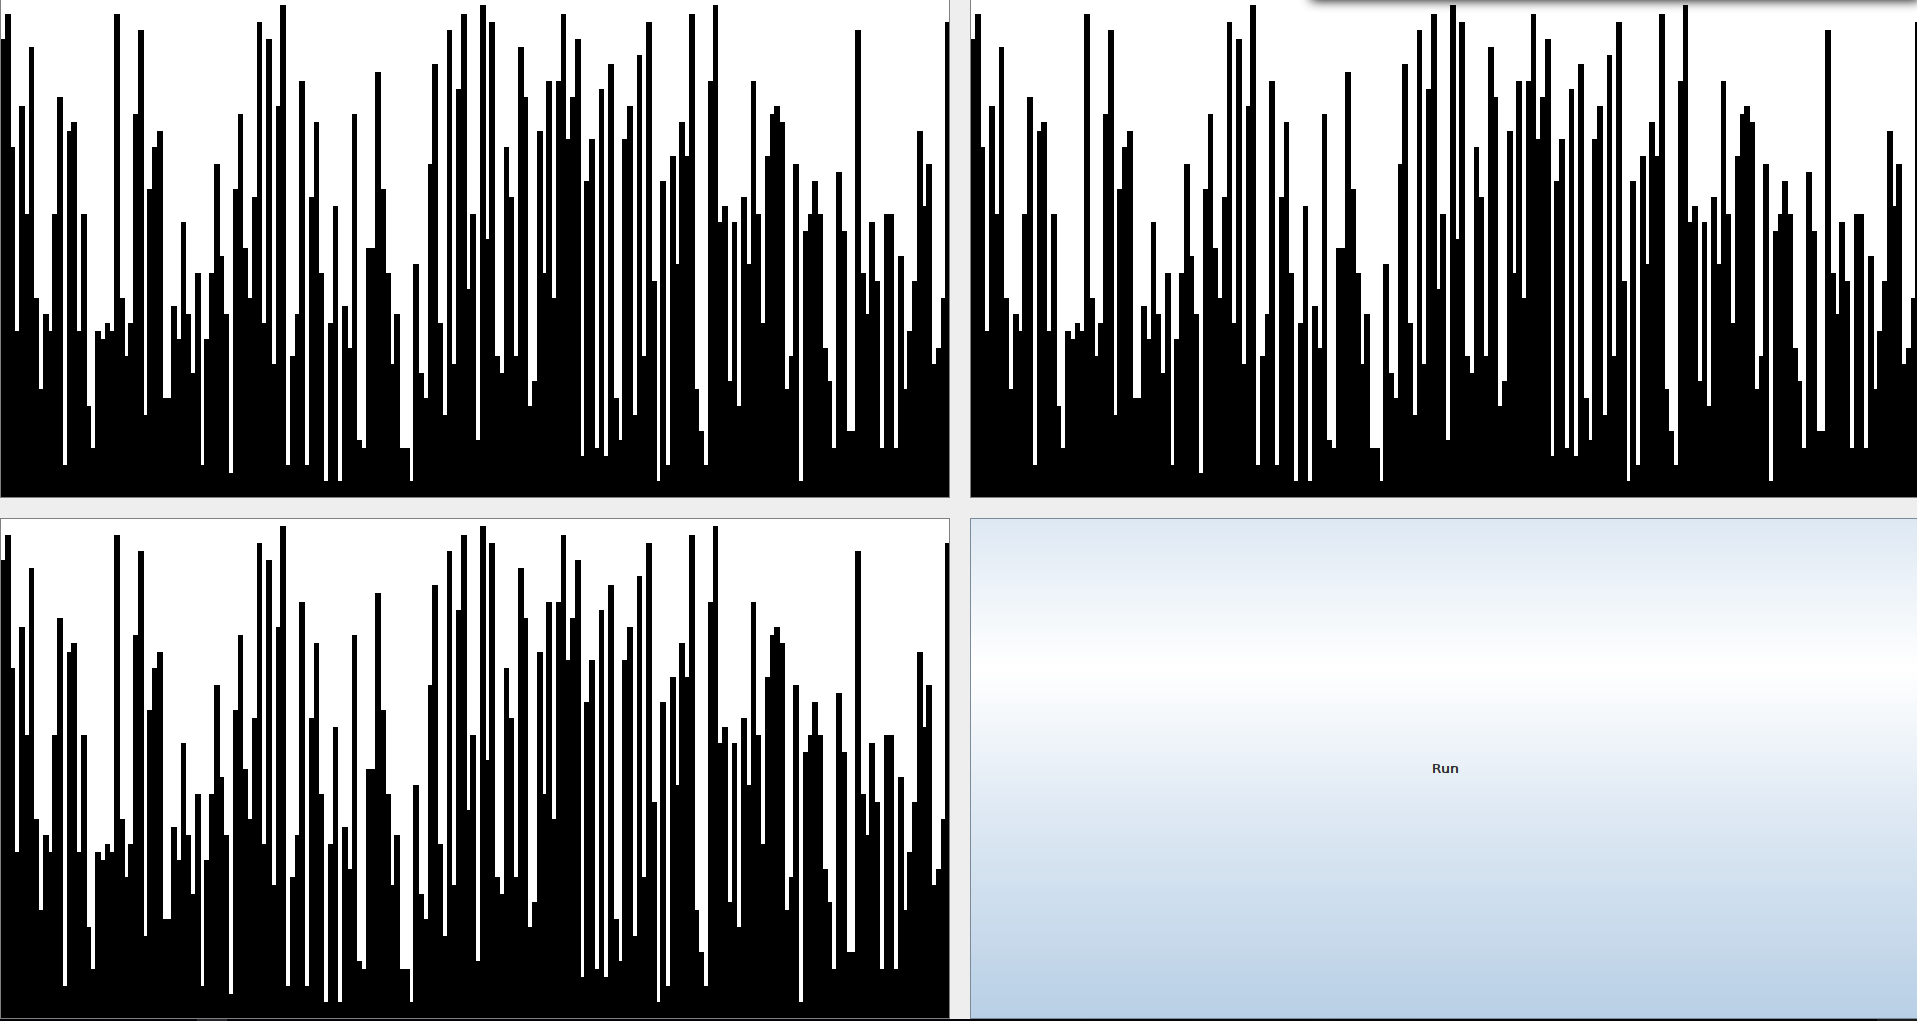
\includegraphics[width=\linewidth]{Layout.png}
    \caption{Esquema de la visualización gráfica.}
\end{figure}

El código que sigue corresponde a la clase Panel mencionada anteriormente, y simplemente crea el contenedor.

\begin{lstlisting}


import java.awt.Color;
import java.awt.GridLayout;
import javax.swing.BorderFactory;
import javax.swing.JButton;
import javax.swing.JFrame;

public class Panel extends JFrame {

    private int stepTime;
    private int numElems;
    private int[] elems;

    private int[] crearArr(int n) {
        int[] result = new int[n];
        for (int i = 0; i < n; i++) {
            result[i] = ((int) (Math.random() * 58)) + 2;
        }
        return result;
    }

    public Panel(int stepTime, int numElems) {
        super("Visualization");
        this.stepTime = stepTime;
        this.numElems = numElems;
        this.elems = crearArr(numElems);

        this.setLayout(new GridLayout(0, 2, 20, 20));
        this.setDefaultCloseOperation(JFrame.EXIT_ON_CLOSE);
        this.setResizable(false);
        this.setExtendedState(MAXIMIZED_BOTH);
        this.setVisible(true);


        GPanel panel1 = new GPanel(elems, stepTime);
        panel1.setBorder(BorderFactory.createLineBorder(Color.GRAY));
        panel1.setBackground(Color.WHITE);

        GPanel panel2 = new GPanel(elems, stepTime);
        panel2.setBorder(BorderFactory.createLineBorder(Color.GRAY));
        panel2.setBackground(Color.WHITE);

        GPanel panel3 = new GPanel(elems, stepTime);
        panel3.setBorder(BorderFactory.createLineBorder(Color.GRAY));
        panel3.setBackground(Color.WHITE);

        JButton startButton = new JButton("Run");
        startButton.addActionListener(e -> {
            panel1.sortAsync(InsertionSort(elems));
            panel2.sortAsync(BubbleSort(elems));
            panel3.sortAsync(SelectionSort(elems));
        });

        add(panel1);
        add(panel2);
        add(panel3);
        add(startButton);

    }

}


\end{lstlisting}

La clase GPanel es la clase que dibuja el gráfico de los elementos, y se muestra a continuación:


\begin{lstlisting}

package lab4.java;

import java.awt.Color;
import java.awt.Graphics;
import java.awt.Graphics2D;
import java.awt.geom.Rectangle2D;
import javax.swing.JPanel;
import javax.swing.Timer;

public class GPanel extends JPanel {

    private int[] elems;
    int stepTime;

    private Rectangle2D[] squares = new Rectangle2D[elems.length];
    private boolean inicializado = false;
    private double heightRatio = this.getHeight() / 60.0;
    private double widthRatio  = this.getWidth()  / 50.0;

    public GPanel(int[] elems, int stepTime) {
        this.elems = elems;
        this.stepTime = stepTime;

    }

    public void swap(int i, int j) {
        inicializado = true;
        double minH = squares[i].getMinX();
        squares[i].setRect(squares[j].getMinX(), squares[i].getMinY(), 30, squares[i].getHeight());
        squares[j].setRect(minH, squares[j].getMinY(), 30, squares[j].getHeight());

        //change position of shapes in array
        Rectangle2D temp = squares[i];
        squares[i] = squares[j];
        squares[j] = temp;
        this.repaint();

    }


    void sortAsync(SortAlgorithm algo) {

        Timer t = null;
        t = new Timer(stepTime) {
            if (!algo.isSorted()) {
                algo.step((i, j) -> swap(i, j));
            } else {
                System.out.println("Stopping timer from ${Thread.currentThread().name}");
                assert t != null;
                t.stop();
            }
        };
        t.start();

    }

    public void paintComponent(Graphics g) {
        super.paintComponent(g);
        Graphics2D ga = (Graphics2D) g;

        heightRatio = this.getHeight() / 60.0;
        widthRatio  = (double) this.getWidth()  / elems.length;

        if (!inicializado) {

            for (int i = 0; i < elems.length; i++) {
                double elemHeight = elems[i] * heightRatio;
                squares[i] = new Rectangle2D.Double(
                        i * widthRatio,
                        this.getHeight() - elemHeight,
                        widthRatio,
                        elemHeight
                );
                ga.draw(squares[i]);
                ga.setColor(Color.BLACK);
                ga.fill(squares[i]);
            }
        }


    }


}


\end{lstlisting}

Aquí se crea un array de Rectangle2D, los cuales son las barras de la gráfica.

Además, en esta clase se encuentra el código responsable de manejar la visualización,
por lo que amerita explicarlo.

\subsection{Hilos de ejecución}

Como ya vimos, existen varios de estos gráficos a la vez, y cada uno de ellos ejecutará un algoritmo
distinto. Esto implica que es necesario usar varios nucleos/hilos del procesador, sin embargo eso no es
posible al trabajar con librerías gráficas.

El método sortAsync se llama cuando se inicia a ordenar el gráfico, toma como parametro una clase
SortAlgorithm que contiene el algoritmo a realizar. Sin embargo, pasar simplemente el algoritmo impide que
se aprovechen los nucleos del procesador, y no es posible usar la clase Thread con gráficos.

Para ello se usa la clase Timer, esta ejecuta una función cada cierto tiempo (en este caso el algoritmo
de ordenamiento) de forma paralela, permitiendo la visualización.

\begin{lstlisting}

public void swap(int i, int j) {
    inicializado = true;
    double minH = squares[i].getMinX();
    squares[i].setRect(squares[j].getMinX(), squares[i].getMinY(), 30, squares[i].getHeight());
    squares[j].setRect(minH, squares[j].getMinY(), 30, squares[j].getHeight());

    //change position of shapes in array
    Rectangle2D temp = squares[i];
    squares[i] = squares[j];
    squares[j] = temp;
    this.repaint();

}

\end{lstlisting}

El método swap intercambia dos rectangulos de la gráfica, tomando como parametros sus posiciones.

Sin embargo, ya que la implementación es independiente de la gráfica, es necesario permitir que cada
algoritmo de ordenación use este método cuando sea necesario. Para ello se crearon las siguientes
interfaces.

\begin{lstlisting}

public interface SortAlgorithm {

    int[] elems = null;

    void step(Swap s);

    boolean isSorted();

}


public interface Swap {

    public void swap(int i1, int i2);

}


\end{lstlisting}

La interfaz SortAlgorithm define el método step(), el cual realiza un paso del algoritmo de ordenamiento.
Esto es así para poder paralelizar los procesos con la clase Timer mencionada anteriormente.

La interfaz Swap se usa para poder pasar el método swap de la clase GPanel a las clases que heredan de
SortAlgorithm.

\subsection{Algoritmos de ordenamiento}

Finalmente, los algoritmos de ordenamiento. Lo único destacable es que, en vez de realizarse a la vez
estos han sido divididos en una serie de pasos.

\begin{lstlisting}


public class BubbleSort implements SortAlgorithm {

    private int[] elems;
    private int posLoop1 = elems.length - 1;
    private int posLoop2 = 1;

    public BubbleSort(int[] elems) {
        this.elems = elems;
    }

    @Override
    public void step(Swap s) {
        if (elems[posLoop2 - 1] > elems[posLoop2]) {

            s.swap(posLoop2, posLoop2 - 1);
            int temp = elems[posLoop2 - 1];
            elems[posLoop2 - 1] = elems[posLoop2];
            elems[posLoop2] = temp;

        }

        if (posLoop2 == posLoop1) {
            posLoop1--;
            posLoop2 = 1;
        } else {
            posLoop2++;
        }
    }

    @Override
    public boolean isSorted() {
        return posLoop1 == 0;
    }

}


\end{lstlisting}


\begin{lstlisting}


public class InsertionSort implements SortAlgorithm {

    private int[] elems;
    int actualIter = 1;
    int posActual = 1;

    public InsertionSort(int[] elems) {
        this.elems = elems;
    }

    @Override
    public void step(Swap s) {

        if (elems[posActual - 1] > elems[posActual]) {

            s.swap(posActual, posActual - 1);
            int temp = elems[posActual - 1];
            elems[posActual - 1] = elems[posActual];
            elems[posActual] = temp;

            if (posActual == 1) {
                actualIter++;
                posActual = actualIter;
            } else {
                posActual--;
            }

        } else {
            actualIter++;
            posActual = actualIter;
        }
    }

    @Override
    public boolean isSorted() {
        return actualIter == elems.length;
    }

}

\end{lstlisting}

\begin{lstlisting}


public class SelectionSort implements SortAlgorithm {

    private int[] elems;
    private int actualIter = 0;
    private int actualPos = actualIter + 1;
    private int minimumPos = actualIter;

    public SelectionSort(int[] elems) {
        this.elems = elems;
    }

    @Override
    public void step(Swap s) {
        if (elems[actualPos] < elems[minimumPos]) {
            minimumPos = actualPos;
        }

        if (actualPos == elems.length - 1) {
            if (actualIter != minimumPos) {
                s.swap(actualIter, minimumPos);
                int temp = elems[minimumPos];
                elems[minimumPos] = elems[actualIter];
                elems[actualIter] = temp;
            }

            actualIter++;
            actualPos = actualIter + 1;
            minimumPos = actualIter;
        } else {
            actualPos++;
        }

    }

    @Override
    public boolean isSorted() {
        return actualIter == elems.length - 1;
    }

}


\end{lstlisting}

El código completo se encuentra en GitHub: https://github.com/Araozu/ADA/tree/master/src/lab4

\begin{figure}
    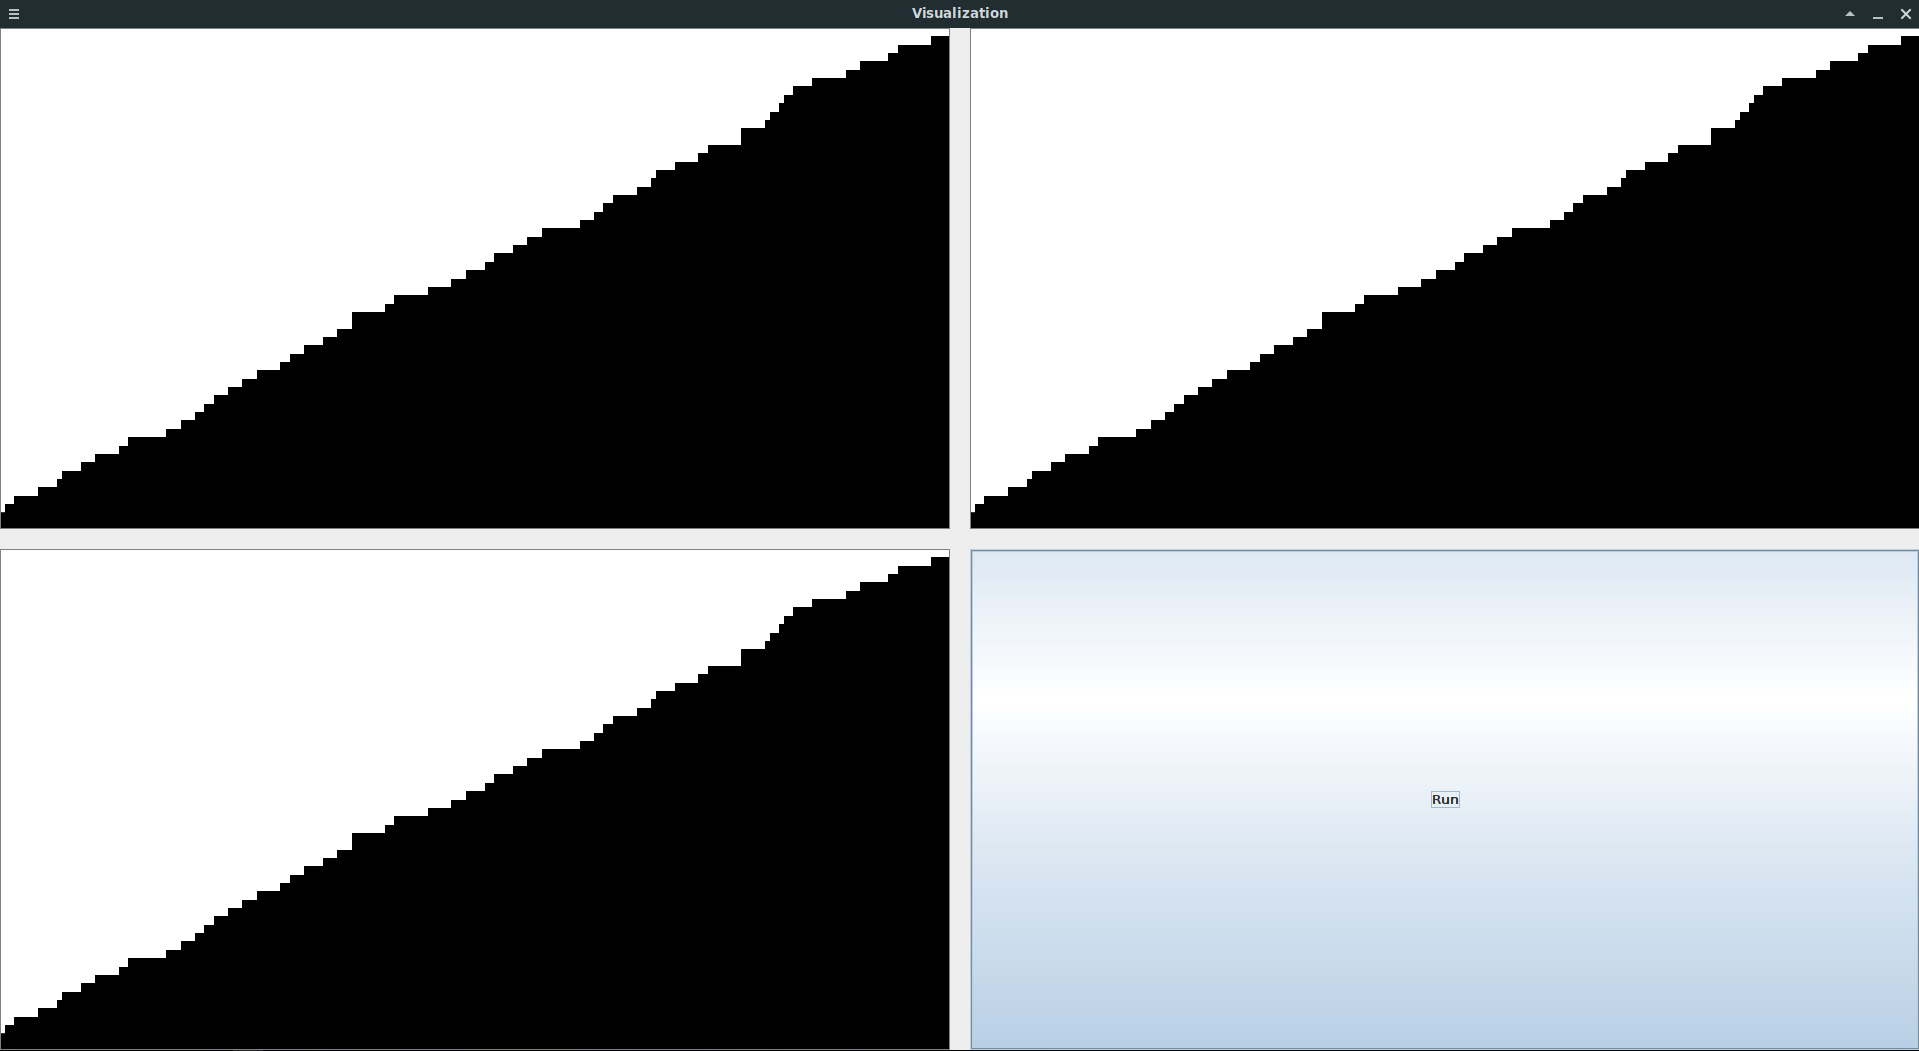
\includegraphics[width=\linewidth]{Resultado.png}
    \caption{Resultado.}
\end{figure}


%------------------------------------------------

\end{document}
